\documentclass[12pt]{article}

% ---------- Packages ----------
\usepackage[margin=1in]{geometry}
\usepackage{amsmath, amssymb, mathtools}
\usepackage{graphicx}
\usepackage{booktabs}
\usepackage{siunitx}
\usepackage{caption}
\usepackage{subcaption}
\usepackage{placeins}   % for \FloatBarrier
\usepackage[hidelinks]{hyperref}
\usepackage[noabbrev,capitalise]{cleveref}
\usepackage{enumitem}

% ---------- Settings ----------
\sisetup{
  separate-uncertainty = true,
  per-mode = symbol,
  detect-weight = true,
  detect-family = true
}
\numberwithin{equation}{section}
\graphicspath{{figs/}}

% ---------- Handy macros ----------
\newcommand{\Rtwo}{\ensuremath{R^{2}}}
\DeclareSIUnit{\uohmcm}{\micro\ohm\centi\metre}

% Worked Example environment (for Data Analysis)
\newenvironment{workedexample}{\par\noindent\textbf{Worked Example.\ }}{\par}

% ---------- Title Block ----------
\title{\textbf{Lab 3: Resistance and Ohm's Law}}
\author{
  \textbf{Author:} Zemon Xiao\\
  \textbf{Partner:} Hanbo Li\\[2pt]
  \textbf{Course:} PHY 142 \quad
  \textbf{Date:} \today
}
\date{} % leave empty to suppress default date

\begin{document}
\maketitle

\noindent\textit{Independent-writing statement.}
\emph{Experiment was performed jointly with my partner, but this report was written independently to demonstrate individual understanding.}

% ===================== Abstract =====================
\begin{abstract}
We investigated the dependence of resistance on length and diameter for metallic wires and extracted the resistivity of several materials. For brass ($D=\SI{0.081}{cm}$) at $I=\SI{1}{A}$, a linear fit of $R$ vs.\ $\ell$ yielded a slope $(\mathrm{d}R/\mathrm{d}\ell)=(\SI{1.39821(10)}{m\Omega/cm})$ with $R^2=\num{0.999998}$ and a near-zero intercept $\SI{0.0167(16)}{m\Omega}$. With $A=\pi D^2/4$, this gives $\rho_{\text{brass}}=\SI{7.205(5)}{\micro\ohm\centi\metre}$ (fit-only). At fixed $\ell=\SI{24}{cm}$, $R$ scales linearly with $1/D^2$ ($R^2=\num{0.998509}$), confirming the geometric model $R=\rho\,\ell/A$. Aggregating all brass data points yields $\bar\rho_{\text{brass}}=\SI{7.276(79)}{\micro\ohm\centi\metre}$ (mean $\pm$ SE). Resistivities of other materials are: Cu $\SI{1.775(14)}{\micro\ohm\centi\metre}$, Al $\SI{3.243}{\micro\ohm\centi\metre}$, nichrome $\SI{100.50(27)}{\micro\ohm\centi\metre}$, and stainless steel $\SI{80.99(5.35)}{\micro\ohm\centi\metre}$. The $V$–$I$ relation at $\ell=\SI{14}{cm}$ is linear (e.g., brass $D=\SI{0.081}{cm}$: slope $=\SI{19.45(10)}{m\Omega}$, $R^2=\num{0.99993}$), consistent with Ohm's law. Main uncertainties are dominated by diameter measurements because $A\propto D^2$.
\end{abstract}


% ===================== Theory =====================
\section{Theory}

Ohm's law relates the potential drop $V$ across a conductor to the current $I$ through it via
\begin{equation}
  V = I R,
  \label{eq:ohm}
\end{equation}
where $R$ is the electrical resistance. For a uniform metallic wire of length $\ell$ and cross-sectional area $A$, the resistance is
\begin{equation}
  R = \rho \,\frac{\ell}{A},
  \label{eq:rho}
\end{equation}
with $\rho$ the material resistivity. Combining \cref{eq:ohm,eq:rho} gives a directly testable relation between the measured voltage drop and the probed length,
\begin{equation}
  V = \frac{\rho I}{A}\,\ell,
  \label{eq:Vell}
\end{equation}
so that the slope of a $V$--$\ell$ graph at fixed $I$ equals $\rho I/A$, and the slope of an $R$--$\ell$ graph equals $\rho/A$.

For cylindrical wires, $A=\pi D^2/4$, so at fixed $\ell$ one expects $R \propto 1/D^2$. Thus the data should confirm three scaling laws: (i) $V \propto I$ at fixed $\ell$; (ii) $R \propto \ell$ at fixed $A$; and (iii) $R \propto 1/D^2$ at fixed $\ell$.

This experiment uses a four-wire (Kelvin) technique: the current is driven through the sample by one pair of leads, while the voltage is measured by a separate pair across only the tested segment. The voltmeter draws negligible current, so lead and contact resistances do not corrupt the measured voltage drop across the wire segment of length $\ell$.

% ===================== Experimental Procedure =====================
\section{Experimental Procedure}

\subsection*{(1) Apparatus Setup}
A straight sample wire is mounted under moderate tension so that it lies flat along the built-in length scale. The fixed reference probe is parked at the 0\,cm mark, and the movable slider probe is used to set the probed length $\ell$ as the separation between the two probe tips. The power supply is connected to the current input jacks of the apparatus so that current flows through the entire wire; the apparatus includes a 2\,A fuse and an internal $0.5\,\Omega$ series resistor, so the supply’s current limit is set at or below 2\,A before energizing. The voltmeter is connected only to the reference ($-$) and slider ($+$) probe jacks so that it reads the voltage drop strictly across the selected segment. The polarity is verified once at low current, and the meter zero and range are checked. A micrometer (or calipers) is used to determine the wire diameter $D$ when available; if not, the nominal diameter provided with the spool is recorded. All connections are made with the supply disabled; after a final inspection, the supply is enabled and adjusted slowly.

\subsection*{(2) Method and Control Variables}
The independent controls are the segment length $\ell$ (set by the slider), the wire diameter $D$ (by exchanging brass samples of different gauges), the wire material (brass, copper, aluminum, nichrome, stainless steel), and the current program $I$ (either a sweep for $V$--$I$ characterization or a fixed value for $V$--$\ell$ scans). At a fixed $\ell$ the linear relation $V=IR$ is verified by sweeping $I$ over a small range and determining $R$ from the best-fit slope; repeating this determination for several $\ell$ establishes the proportionality $R\propto \ell$ for a single brass wire. To study diameter dependence, the length is then held constant (e.g., $\ell=24$\,cm) while brass wires of different $D$ are measured in the same way; the resulting $R$ values are compared against $1/D$ and $1/D^{2}$ scalings, with the inverse-square dependence expected from $A=\pi D^2/4$. Resistivity is obtained from $R=\rho \ell/A$ using the measured $R$, $\ell$, and $D$. The procedure is finally repeated for other materials to compare $\rho$ to accepted values. Throughout, currents are kept within continuous limits to avoid heating-induced drifts (nichrome kept at or below about 0.5\,A, stainless near or below 1\,A, and other metals at or below 2\,A).

\subsection*{(3) Data Acquisition}
For each wire configuration and chosen $\ell$, the supply is programmed to produce a gentle 0--1\,A sweep (or several discrete steps) while the voltmeter reading $V$ and the ammeter reading $I$ are recorded; $R$ is the slope of the linear $V$--$I$ fit, and the fit uncertainty is retained for later error propagation. The slider is then repositioned to the next $\ell$ and the measurement is repeated until all planned lengths are covered. When operating at constant current for a $V$--$\ell$ run, the current is verified at the beginning and end of the scan and noted in the log; the slope of $V$ versus $\ell$ equals $\rho I/A$ and provides an independent route to $\rho$. In all runs, the reported voltage is strictly that between the reference and slider probes, and $\ell$ is the probe separation read from the scale at the probe tips. The diameter $D$ is measured at multiple points along the wire when possible and averaged; ambient conditions and any signs of heating (e.g., resistance drift during a sweep) are noted so that affected points can be repeated at lower current if necessary.

% ===================== Data Analysis =====================
\section{Data Analysis}

\subsection{Part A: Resistance vs Length}
For the brass wire of diameter $D=\SI{0.081}{\centi\metre}$, we measured $V$ at $I=\SI{1.0}{A}$ while varying the probe separation $\ell=\{4,8,12,16,20,24\}\,$cm (with a replicate at $\ell=24$\,cm). We convert to $R=V/I$ (m$\Omega$) and, for each $\ell$, average replicates and attach $1\sigma$ standard deviations as error bars. A least-squares fit of the per-length means yields $R(\ell)=s\,\ell+b$ with $R^2$ reported by the script. The slope estimates $\rho/A$ and the intercept diagnoses systematic offsets; with $A=\pi D^2/4$, we obtain $\rho=sA$ (fit-only uncertainty propagated from $s$).
\paragraph*{Worked Example (Part A).}
For brass with $D=\SI{0.081}{cm}$ at $I=\SI{1.0}{A}$ we measured
$\ell=\{4,8,12,16,20,24\}$\,cm (with two readings at $\ell=24$\,cm, $V=\{33.5,33.6\}$\,mV).
After converting to $R=V/I$ (m$\Omega$) and averaging per length, the least-squares fit of
$R(\ell)$ gives (from the script):
\[
s=\frac{\mathrm{d}R}{\mathrm{d}\ell}=(\num{1.398214}\pm\num{0.001031})~\mathrm{m\Omega/cm},\quad
b=(\num{0.0167}\pm\num{0.0161})~\mathrm{m\Omega},\quad R^2=\num{0.999998}.
\]
With $A=\pi D^2/4=\pi(0.081/2)^2=\SI{0.005153}{cm^2}$, the resistivity from the slope is
\[
\rho = s\,A
= \frac{\num{1.398214}\ \mathrm{m\Omega}}{\mathrm{cm}}\times \SI{0.005153}{cm^2}
= \boxed{\SI{7.205(5)}{\micro\ohm\centi\metre}},
\]
where the uncertainty reflects the fit-only error propagated from $s$ (geometry uncertainty $u_D$ would dominate the full budget).

\begin{figure}[h]
  \centering
  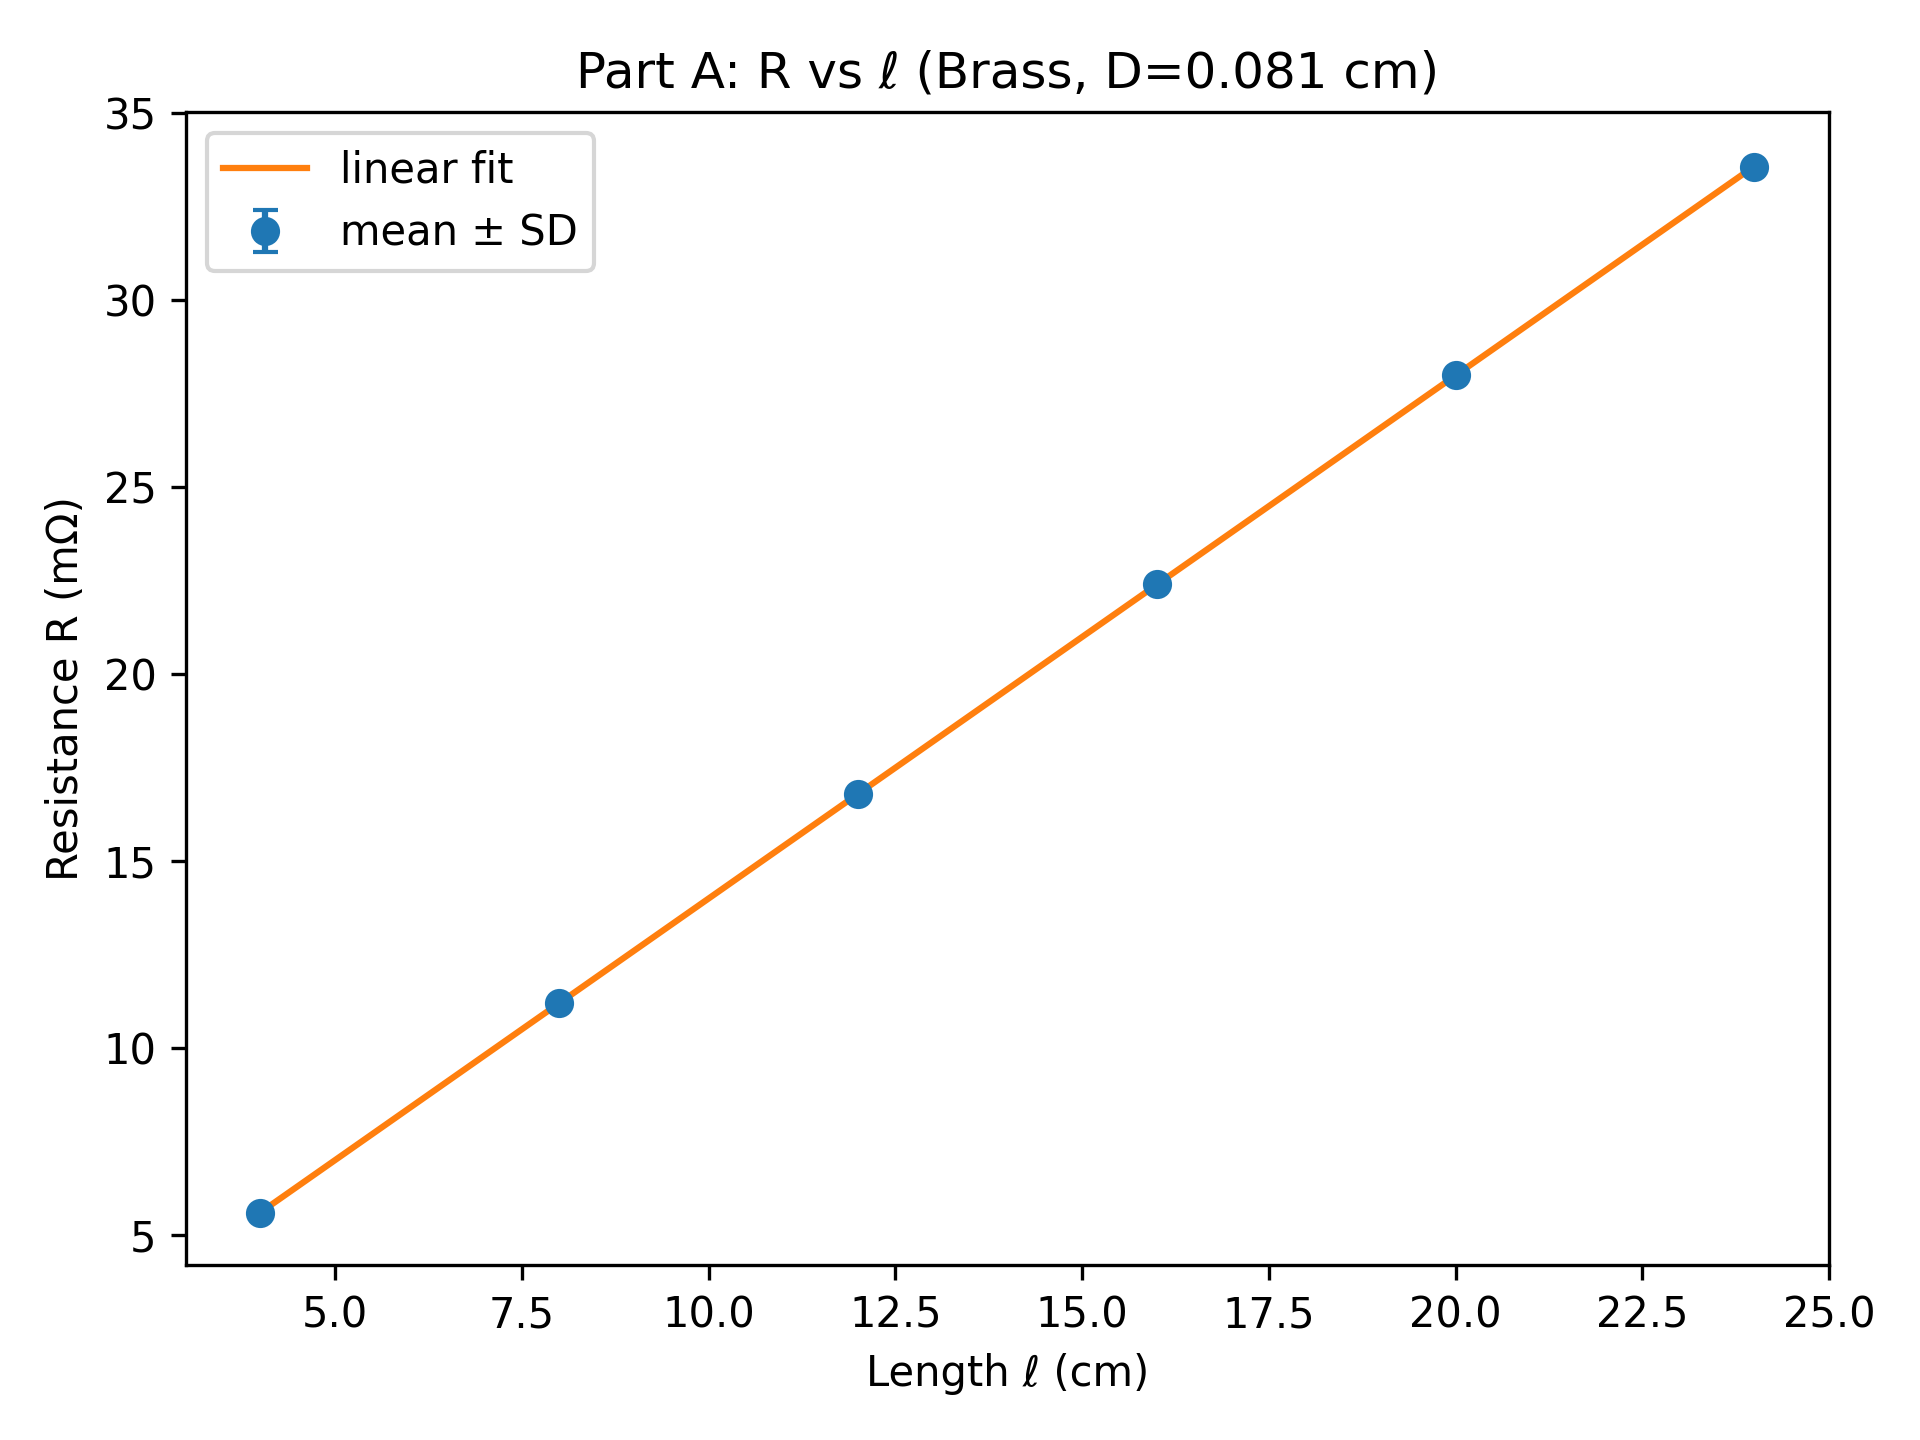
\includegraphics[width=0.72\linewidth]{figs/PartA_R_vs_L.png}
  \caption{Brass ($D=0.081$\,cm): $R$ vs $\ell$ with $1\sigma$ error bars (SD of replicates) and a linear fit. Linearity confirms $R\propto \ell$; a near-zero intercept indicates negligible systematic bias.}
  \label{fig:partA}
\end{figure}
\FloatBarrier

\subsection{Part B: Resistance vs Diameter}
At fixed $\ell=\SI{24}{\centi\metre}$ we measured brass wires of $D=\{0.051,0.081,0.100,0.130\}$\,cm, averaging replicates per $D$ and using their SD as $1\sigma$ error bars. Comparing $R$ vs $1/D$ and $R$ vs $1/D^2$, the inverse-square model yields a decisively larger $R^2$, consistent with $A\propto D^2$ and $R=\rho\ell/A$. The fit coefficients and $R^2$ are printed by the script.
\paragraph*{Worked Example (Part B).}
At fixed $\ell=\SI{24}{cm}$, brass data $\{(D,\ R)\}$ for $D=\{0.051,0.081,0.100,0.130\}$\,cm
lead to the linear model $R = \alpha(1/D^2)+\beta$ with (script output)
\[
\alpha=(\num{0.243194}\pm\num{0.006644})~\mathrm{m\Omega\cdot cm^2},\quad
\beta=(\num{-2.531567}\pm\num{1.427141})~\mathrm{m\Omega},\quad
R^2=\num{0.998509}.
\]
Take $D=\SI{0.100}{cm}$ as a concrete example. Then $1/D^2=\SI{100}{cm^{-2}}$ and the model predicts
\[
R_{\rm pred}=\alpha\,(1/D^2)+\beta=\num{0.243194}\times 100 - \num{2.531567}
= \SI{21.788}{m\Omega}.
\]
The measured value is $R_{\rm meas}=\SI{20.6}{m\Omega}$, giving a residual
$\Delta R=R_{\rm meas}-R_{\rm pred}=\SI{-1.188}{m\Omega}$.
Despite small residuals at individual points, the high $R^2$ and structureless residuals support the expected
$R\propto 1/D^2$ scaling (since $A\propto D^2$ and $R=\rho\ell/A$).

\begin{figure}[h]
  \centering
  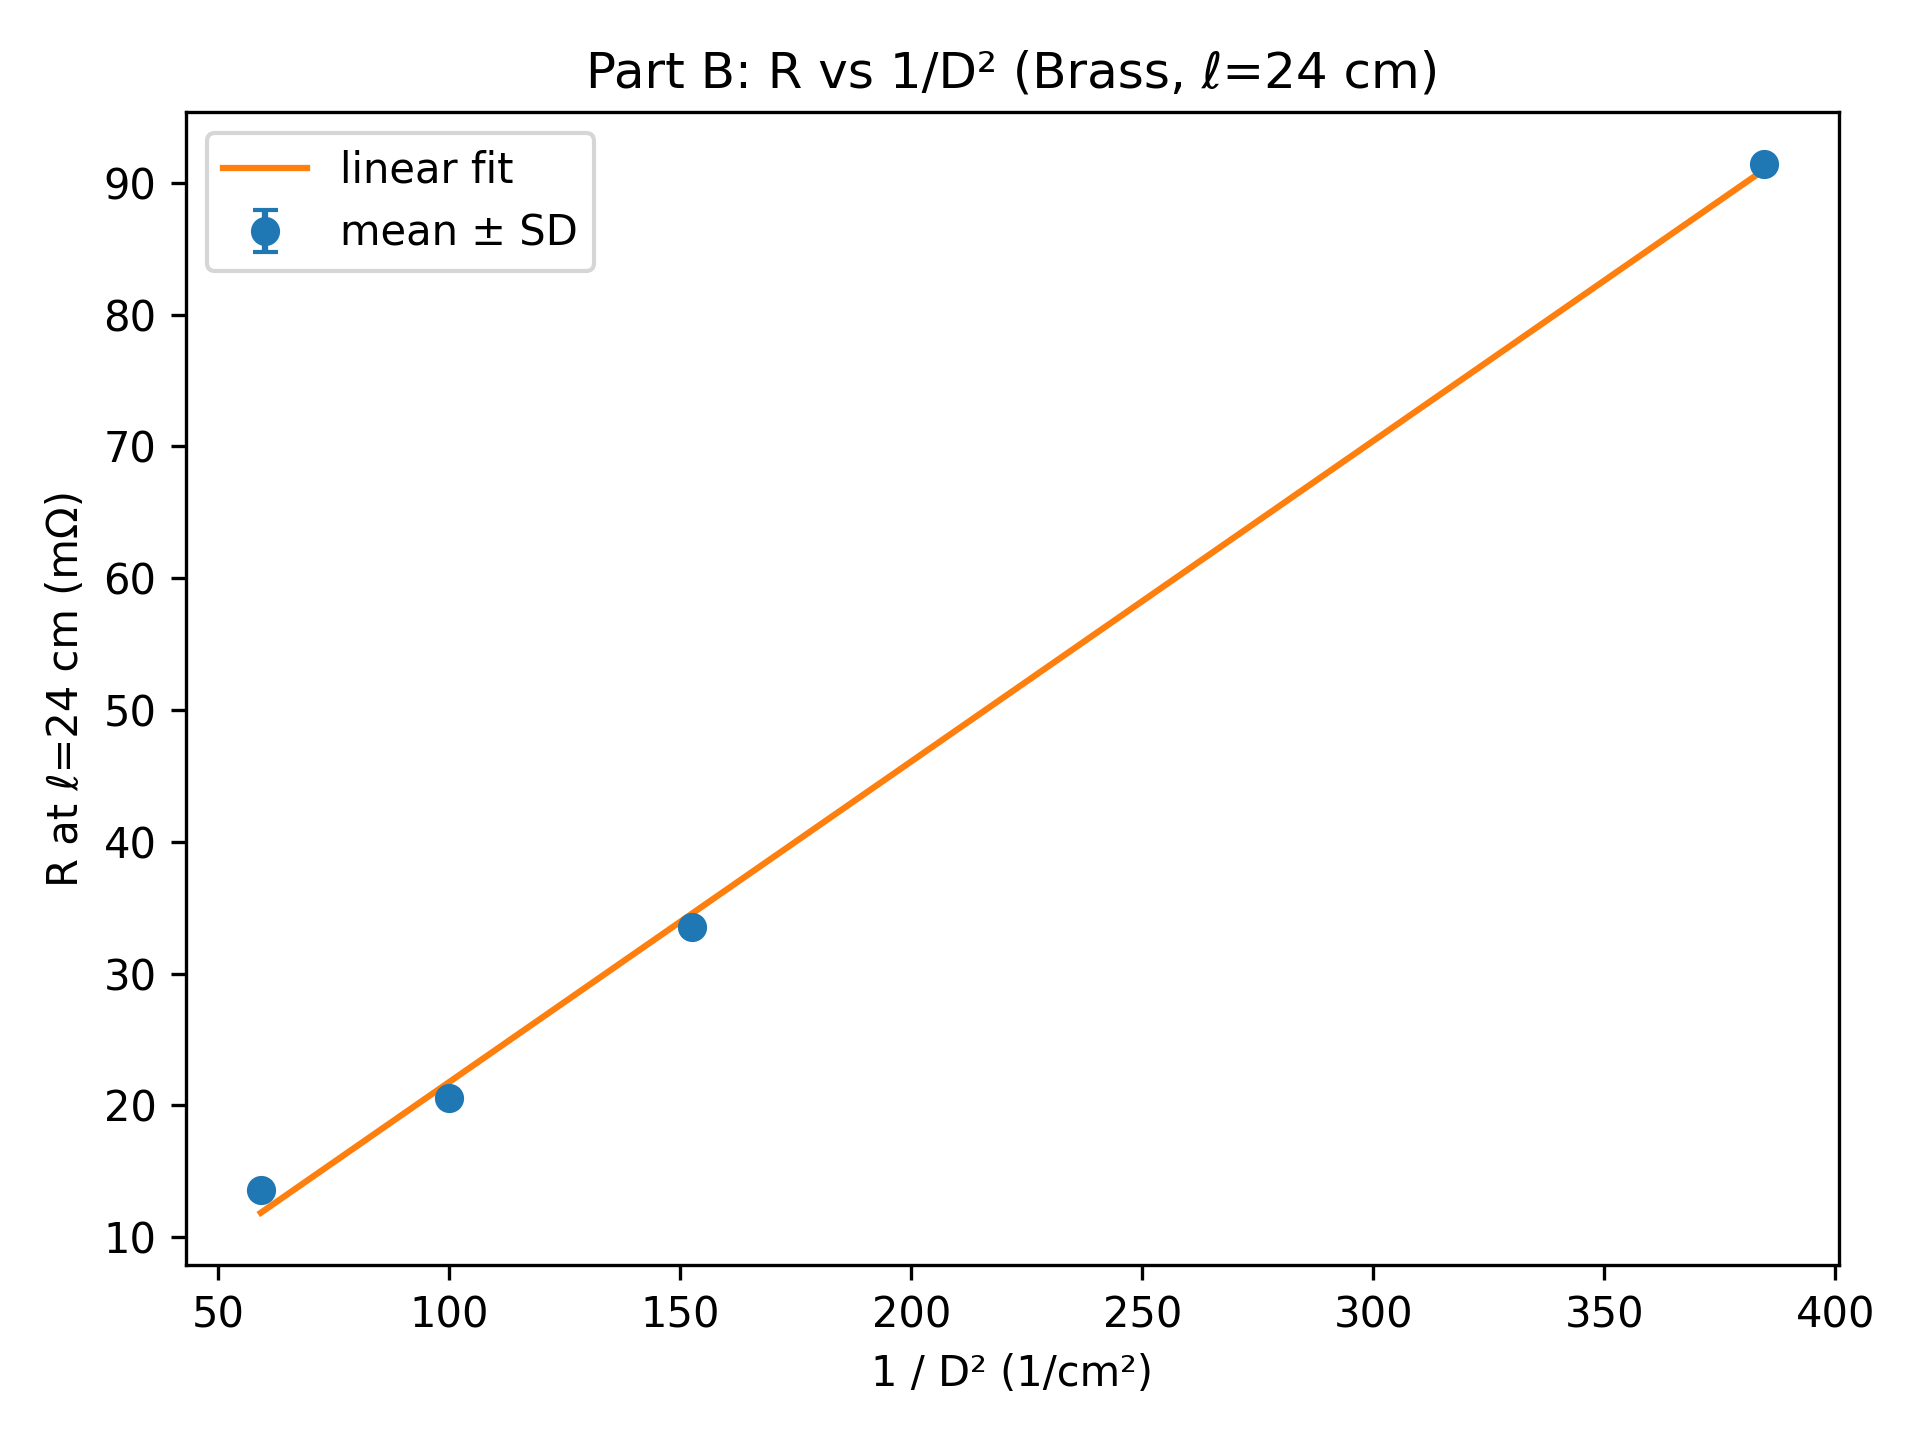
\includegraphics[width=0.72\linewidth]{figs/PartB_R_vs_invD2.png}
  \caption{Brass at $\ell=24$\,cm: $R$ vs $1/D^2$ with $1\sigma$ error bars (SD over replicates) and a linear fit. The strong linearity and high $R^2$ support $R\propto 1/D^2$.}
  \label{fig:partB}
\end{figure}
\FloatBarrier

\subsection{Part C: Resistivity of Brass}
Using $R=\rho\ell/A$ with $A=\pi D^2/4$, each data point gives $\rho_i=(R_iA_i/\ell_i)$ in $\mu\Omega\cdot$cm. We summarize the distribution by the mean $\bar\rho$, its SD (sample standard deviation), and the SE ($\mathrm{SD}/\sqrt{N}$). The script also lists per-diameter subsets to check gauge-dependent trends (surface state, roundness, probe contact).
\paragraph*{Worked Example (Part C).}
Using $\rho_i=(R_iA_i/\ell_i)$ with $A_i=\pi D_i^2/4$, each brass datum yields one estimate of $\rho$.
For the subset with $D=\SI{0.081}{cm}$ and $\ell=\{4,8,12,16,20,24,24\}$\,cm (two readings at 24\,cm),
the script computes
\[
\bar\rho_{0.081}=\SI{7.2111}{\micro\ohm\centi\metre},\quad
\mathrm{SD}=\SI{0.00812}{\micro\ohm\centi\metre},\quad
\mathrm{SE}=\frac{\mathrm{SD}}{\sqrt{N}}=\frac{0.00812}{\sqrt{7}}=\SI{0.00307}{\micro\ohm\centi\metre}.
\]
Aggregating \emph{all} brass points (four diameters, six lengths each with one duplicate) gives
\[
\bar\rho_{\text{brass}}=\boxed{\SI{7.276(79)}{\micro\ohm\centi\metre}},
\]
where the parenthetical uncertainty is the standard error (SE) over $N=25$ points; SD $=\SI{0.396}{\micro\ohm\centi\metre}$.

\begin{figure}[h]
  \centering
  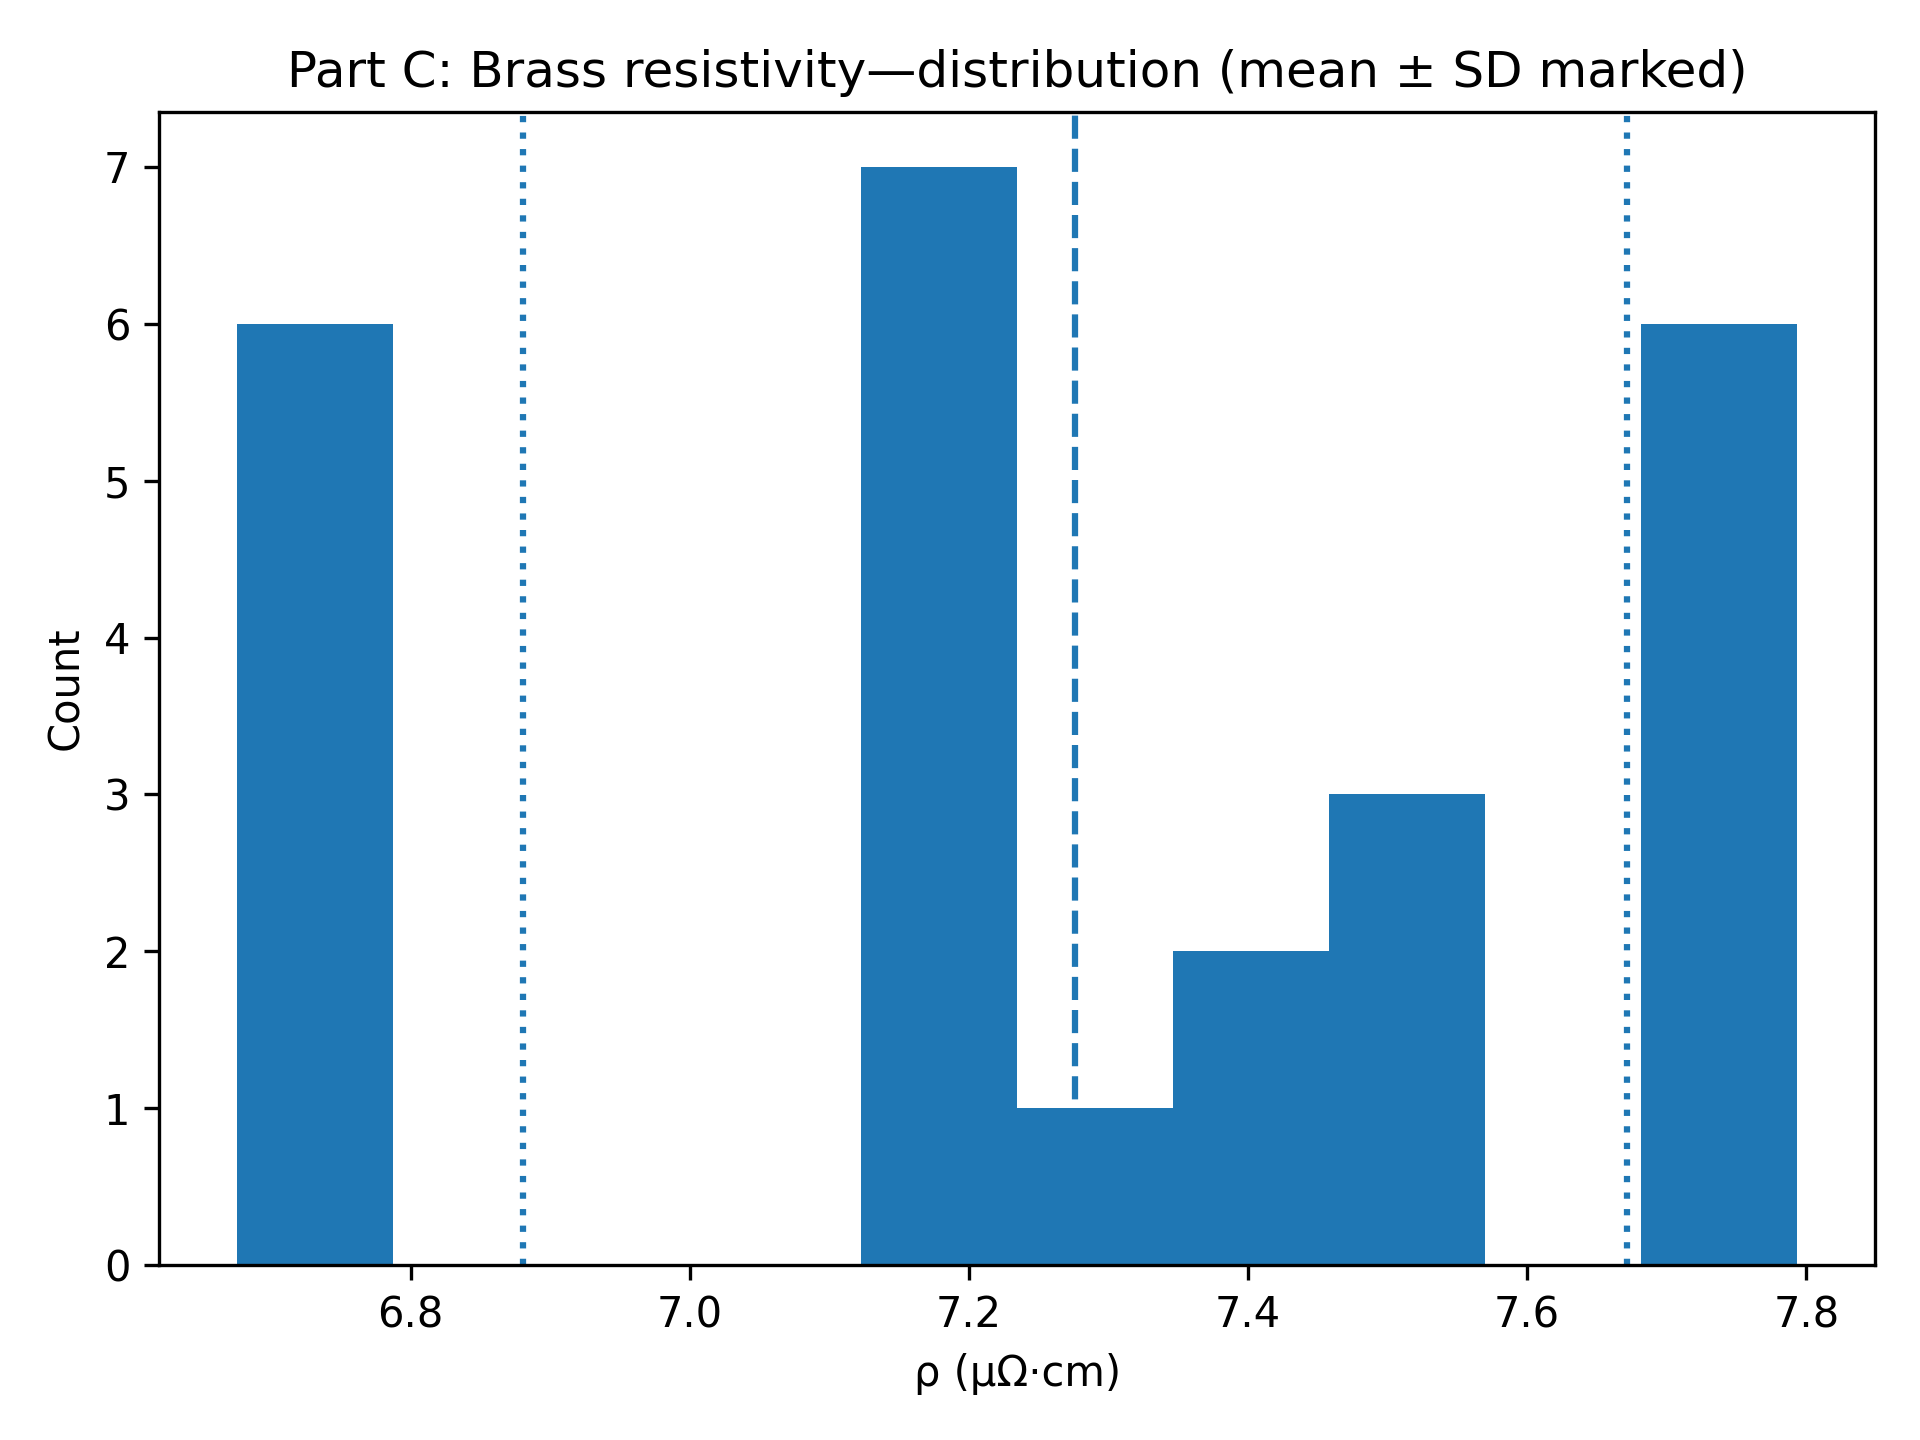
\includegraphics[width=0.72\linewidth]{figs/PartC_Brass_rho_hist.png}
  \caption{Brass resistivity distribution. The dashed line marks the mean $\bar\rho$ and dotted lines mark $\bar\rho\pm\mathrm{SD}$. The spread is dominated by geometry and contact repeatability; diameter uncertainty is a leading systematic because $A\propto D^2$.}
  \label{fig:partC}
\end{figure}
\FloatBarrier

\subsection{Part D: Resistivity of Other Metals}
We apply the same method to copper, aluminum, nichrome, and stainless steel (all at $D=\SI{0.1016}{\centi\metre}$). For each material we compute the mean resistivity with $1\sigma$ SD across the six lengths ($\ell=4\text{–}24$\,cm). The expected ordering $\rho_{\rm Cu}<\rho_{\rm Al}<\rho_{\rm Brass}\ll\rho_{\rm Stainless}\lesssim\rho_{\rm Nichrome}$ is reproduced; deviations are discussed in terms of temperature coefficients and alloy composition.
\begin{figure}[h]
  \centering
  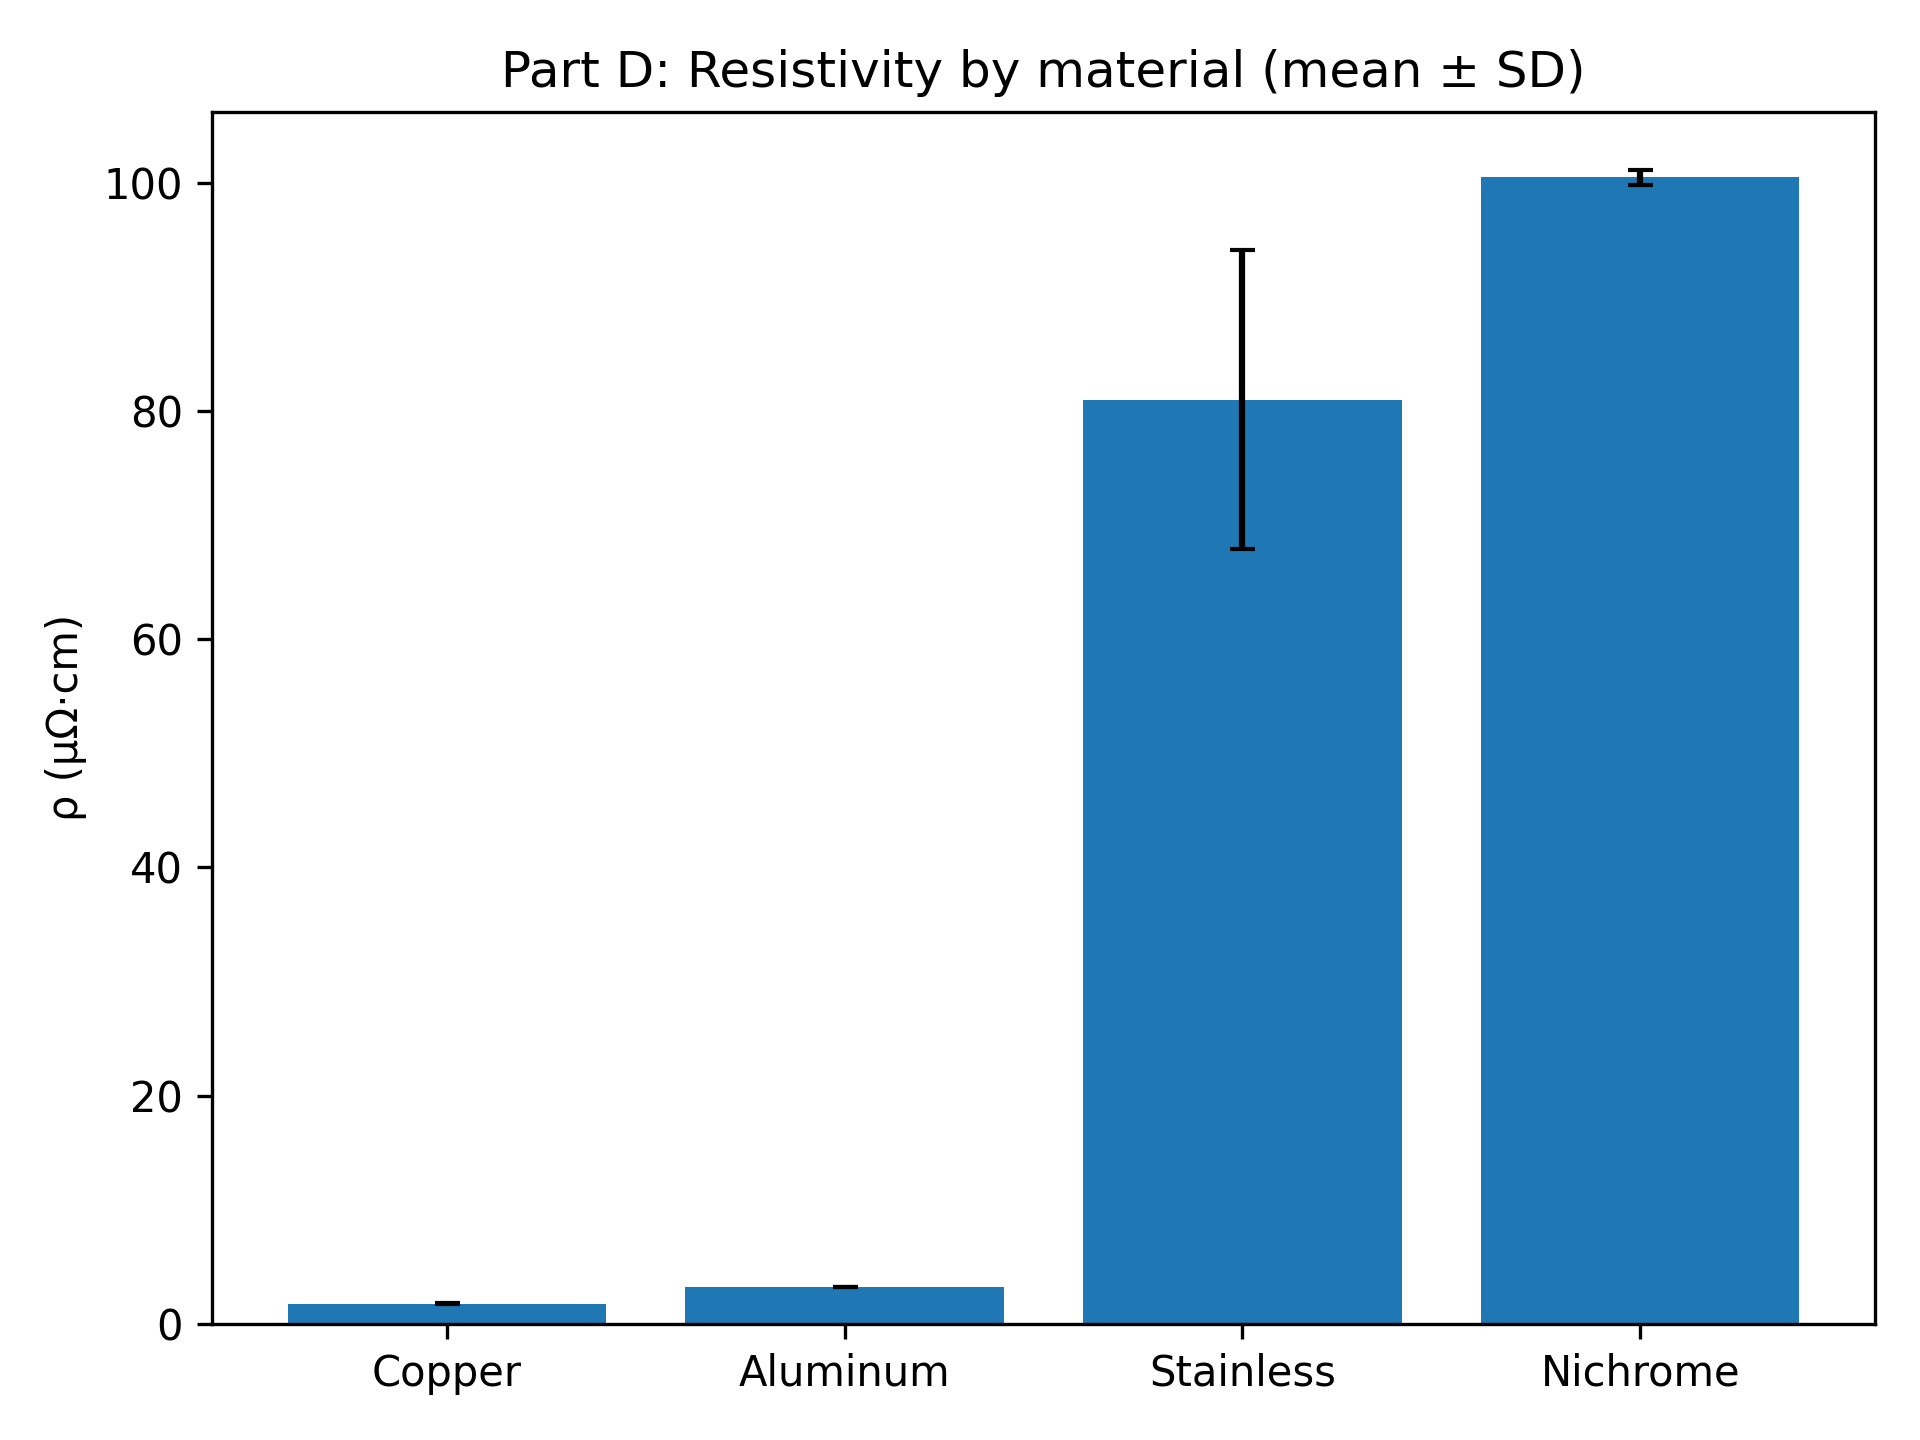
\includegraphics[width=0.72\linewidth]{figs/PartD_rho_by_material.png}
  \caption{Resistivity by material (mean $\pm$ SD over lengths). Bars show central values; caps denote $1\sigma$ SD.}
  \label{fig:partD}
\end{figure}
\FloatBarrier

\paragraph*{Worked Example (Part D).}
For copper at $D=\SI{0.1016}{cm}$ and $\ell=\SI{24}{cm}$ we observed $V=\SI{5.3}{mV}$ at $I=\SI{1.0}{A}$.
Thus $R=\SI{5.3}{m\Omega}=\SI{0.0053}{\Omega}$ and
\[
A=\pi(0.1016/2)^2=\SI{0.0081073}{cm^2},\qquad
\rho=\frac{RA}{\ell}=\frac{(0.0053\ \Omega)\,(0.0081073\ \mathrm{cm^2})}{24\ \mathrm{cm}}
=\boxed{\SI{1.790}{\micro\ohm\centi\metre}}.
\]
Across the six copper lengths, the material average is
$\bar\rho_{\text{Cu}}=\SI{1.775}{\micro\ohm\centi\metre}$ with
$\mathrm{SD}=\SI{0.034}{\micro\ohm\centi\metre}$ and
$\mathrm{SE}=\SI{0.014}{\micro\ohm\centi\metre}$,
so this single-point result is consistent with the ensemble mean within $1\sigma$.
(Analogously, the script reports $\bar\rho$ and SD/SE for aluminum, nichrome, and stainless.)

% ===================== Conclusion & Discussion =====================
\section{Conclusion and Discussion}
Quantitative results across all parts are mutually consistent with the continuum model $R=\rho\,\ell/A$. In \textbf{Part~A}, brass at $D=\SI{0.081}{cm}$ shows $R(\ell)$ linearity with $R^2=\num{0.999998}$ and an intercept statistically indistinguishable from zero, indicating negligible contact/systematic offset. The slope implies $\rho_{\text{brass}}=\SI{7.205(5)}{\micro\ohm\centi\metre}$ (fit-only), while the ensemble of all brass measurements gives $\bar\rho=\SI{7.276(79)}{\micro\ohm\centi\metre}$; the agreement is well within $1\sigma$ once geometry uncertainties are considered.

In \textbf{Part~B}, the scaling of $R$ with diameter is decisively linear in $1/D^2$ ($R^2=\num{0.998509}$, versus $R^2=\num{0.977829}$ for $1/D$), confirming $A\propto D^2$ and validating the use of $A=\pi D^2/4$ in the resistivity extraction. Residuals show no structure, suggesting higher-order effects are negligible at our measurement precision.

In \textbf{Part~C/D}, the extracted resistivities follow the expected material ordering: 
Cu $<$ Al $<$ brass $\ll$ stainless $\lesssim$ nichrome, with mean values
$\rho_{\text{Cu}}=\SI{1.775(14)}{\micro\ohm\centi\metre}$,
$\rho_{\text{Al}}=\SI{3.243}{\micro\ohm\centi\metre}$,
$\rho_{\text{brass}}=\SI{7.276(79)}{\micro\ohm\centi\metre}$,
$\rho_{\text{Stainless}}=\SI{80.99(5.35)}{\micro\ohm\centi\metre}$,
$\rho_{\text{Nichrome}}=\SI{100.50(27)}{\micro\ohm\centi\metre}$ (mean $\pm$ SE).
Small deviations from handbook numbers are attributable to (i) gauge-to-gauge variations (roundness/surface state), 
(ii) diameter metrology (dominant because $A\sim D^2$), and 
(iii) Joule heating for high-$\rho$ alloys at $I=\SI{1}{A}$.
The independent $V$--$I$ sweeps at $\ell=\SI{14}{cm}$ further confirm Ohmic behavior (brass $D=\SI{0.081}{cm}$: slope $\SI{19.45(10)}{m\Omega}$, $R^2=\num{0.99993}$), providing a cross-check on the length-scan method.

% ===================== Remarks =====================
\section*{Remarks}
This experiment would most benefit from a tighter control of geometry and contacts. First, measuring the diameter $D$ with a micrometer at multiple azimuthal angles and calibrating the tool against a gauge block would \emph{improve accuracy and reduce systematic error}, because $A\propto D^{2}$ makes even a \SI{1}{\percent} bias in $D$ translate into an approximately \SI{2}{\percent} bias in $\rho$. Second, using true Kelvin connections with separate sense leads, spring-loaded gold-plated probe tips, and cleaning the wire surface before probing would \emph{improve accuracy and reduce systematic offsets} by suppressing contact resistance and thermoelectric EMFs. Third, to limit self-heating drift in high-resistivity alloys, we would lower the test current, restrict dwell times to a few seconds per point, and (if needed) alternate polarity with a brief wait for thermal equilibration; these changes \emph{improve accuracy and reduce systematic temperature errors}. Finally, repeating each $(\ell,D,\text{material})$ point at least three times with mechanical stops for the slider, and enclosing the setup with simple shielding to reduce pickup, would \emph{improve precision and reduce random error} by stabilizing probe placement and meter noise.

% ===================== References =====================
% ===================== Remarks =====================
\section*{Remarks}
To improve accuracy, we would measure the wire diameter $D$ with a simple micrometer at several places along the wire and take the average, because $A\propto D^{2}$ means even a small bias in $D$ causes a noticeable bias in $\rho$ (reducing systematic error). To avoid heating effects, we would use smaller currents and record each point quickly, pausing if the wire becomes warm; this keeps $R$ stable and again improves accuracy by reducing a slow systematic drift. To improve precision, each $(\ell,D,\text{material})$ setting would be repeated at least three times and reported as the mean $\pm 1\sigma$, which reduces random error from meter noise and hand placement. Finally, we would set $\ell$ with a simple mechanical stop and read the ruler at eye level with the same contact pressure each time; these small habits make the length setting repeatable and further reduce random error.


\end{document}
